% !TeX root = ../main.tex

\section*{\href{http://ieeexplore.ieee.org/document/1000236/?arnumber=1000236&tag=1}{Mean Shift Algorithm}}

\paragraph{Idea:}
Find maxima in pdf without actually performing a full density estimation \footnote{This applies only in some cases, e.g. quickly finding clusters through particle tracing or with a down-sampled PDF}. Maxima can be found, where the gradient of the pdf is zero. \\

Assume that we have a full density estimation
\begin{equation*}
p(\vec{x}) = \dfrac{1}{N} \sum_{i=1}^N k_h(\vec{x}; \vec{x_i})
\end{equation*}
denotes the multivariate kernel density estimation, where we assume $k_h$ to be a radially symmetric kernel, i.e. $k(\vec{x}; \vec{x_i}) = k_h(||\vec{x_i} - \vec{x}||^2)$. A local maximum of the pdf can be assumed where the gradient vanishes 


\begin{align*}
	\nabla p(\vec{x}) &= \dfrac{1}{N} \sum_{i=1}^N \nabla k(\vec{x}; \vec{x_i}) \doteq \vec{0} \\
	\nabla p(\vec{x}) &= \dfrac{1}{N} \sum_{i=1}^N k_h'(||\vec{x_i} - \vec{x}||^2) \cdot (-2 (\vec{x_i} - \vec{x})) \doteq \vec{0}
\end{align*}

All constants can be dropped, then we multiply the kernel with it's derivative

\begin{equation*}
  \sum_{i=1}^N k_h'(||\vec{x_i} - \vec{x}||^2) \vec{x_i} - \sum_{i=1}^N k_h'(||\vec{x_i} - \vec{x}||^2) \vec{x} \doteq \vec{0}
\end{equation*}

Then we get the mean shift vector

\begin{equation*}
  \boxed{\label{mean-shift-vector}
  \Rightarrow m(\vec{x}) = \dfrac{\sum_{i=1}^N k_h'(||\vec{x_i} - \vec{x}||^2) \vec{x_i}}{\sum_{i=1}^N k_h'(||\vec{x_i} - \vec{x}||^2)} - \vec{x} \doteq \vec{0}}
\end{equation*}

To perform a gradient ascent, compute the gradient, walk one step, re-compute the gradient, walk a step, \ldots

\paragraph{Mean Shift Algorithm}
\begin{enumerate}
  \item Compute the mean shift vector $m(\vec{x}^{(t)})$
  \item Update $\vec{x}:\vec{x}^{(t+1)} = \vec{x}^{(t)} + m(\vec{x}^{(t)}) = \vec{x}^{(t)} + \dfrac{\sum_{i=1}^N k_h'(||\vec{x_i} - \vec{x}||^2) \vec{x_i}}{\sum_{i=1}^N k_h'(||\vec{x_i} - \vec{x}||^2)} - \vec{x}^{(t)}= \dfrac{\sum_{i=1}^N k_h'(||\vec{x_i} - \vec{x}||^2) \vec{x_i}}{\sum_{i=1}^N k_h'(||\vec{x_i} - \vec{x}||^2)}$
\end{enumerate}

\begin{figure}[H] 
	\centering
	\begin{minipage}[b]{0.4\textwidth}
		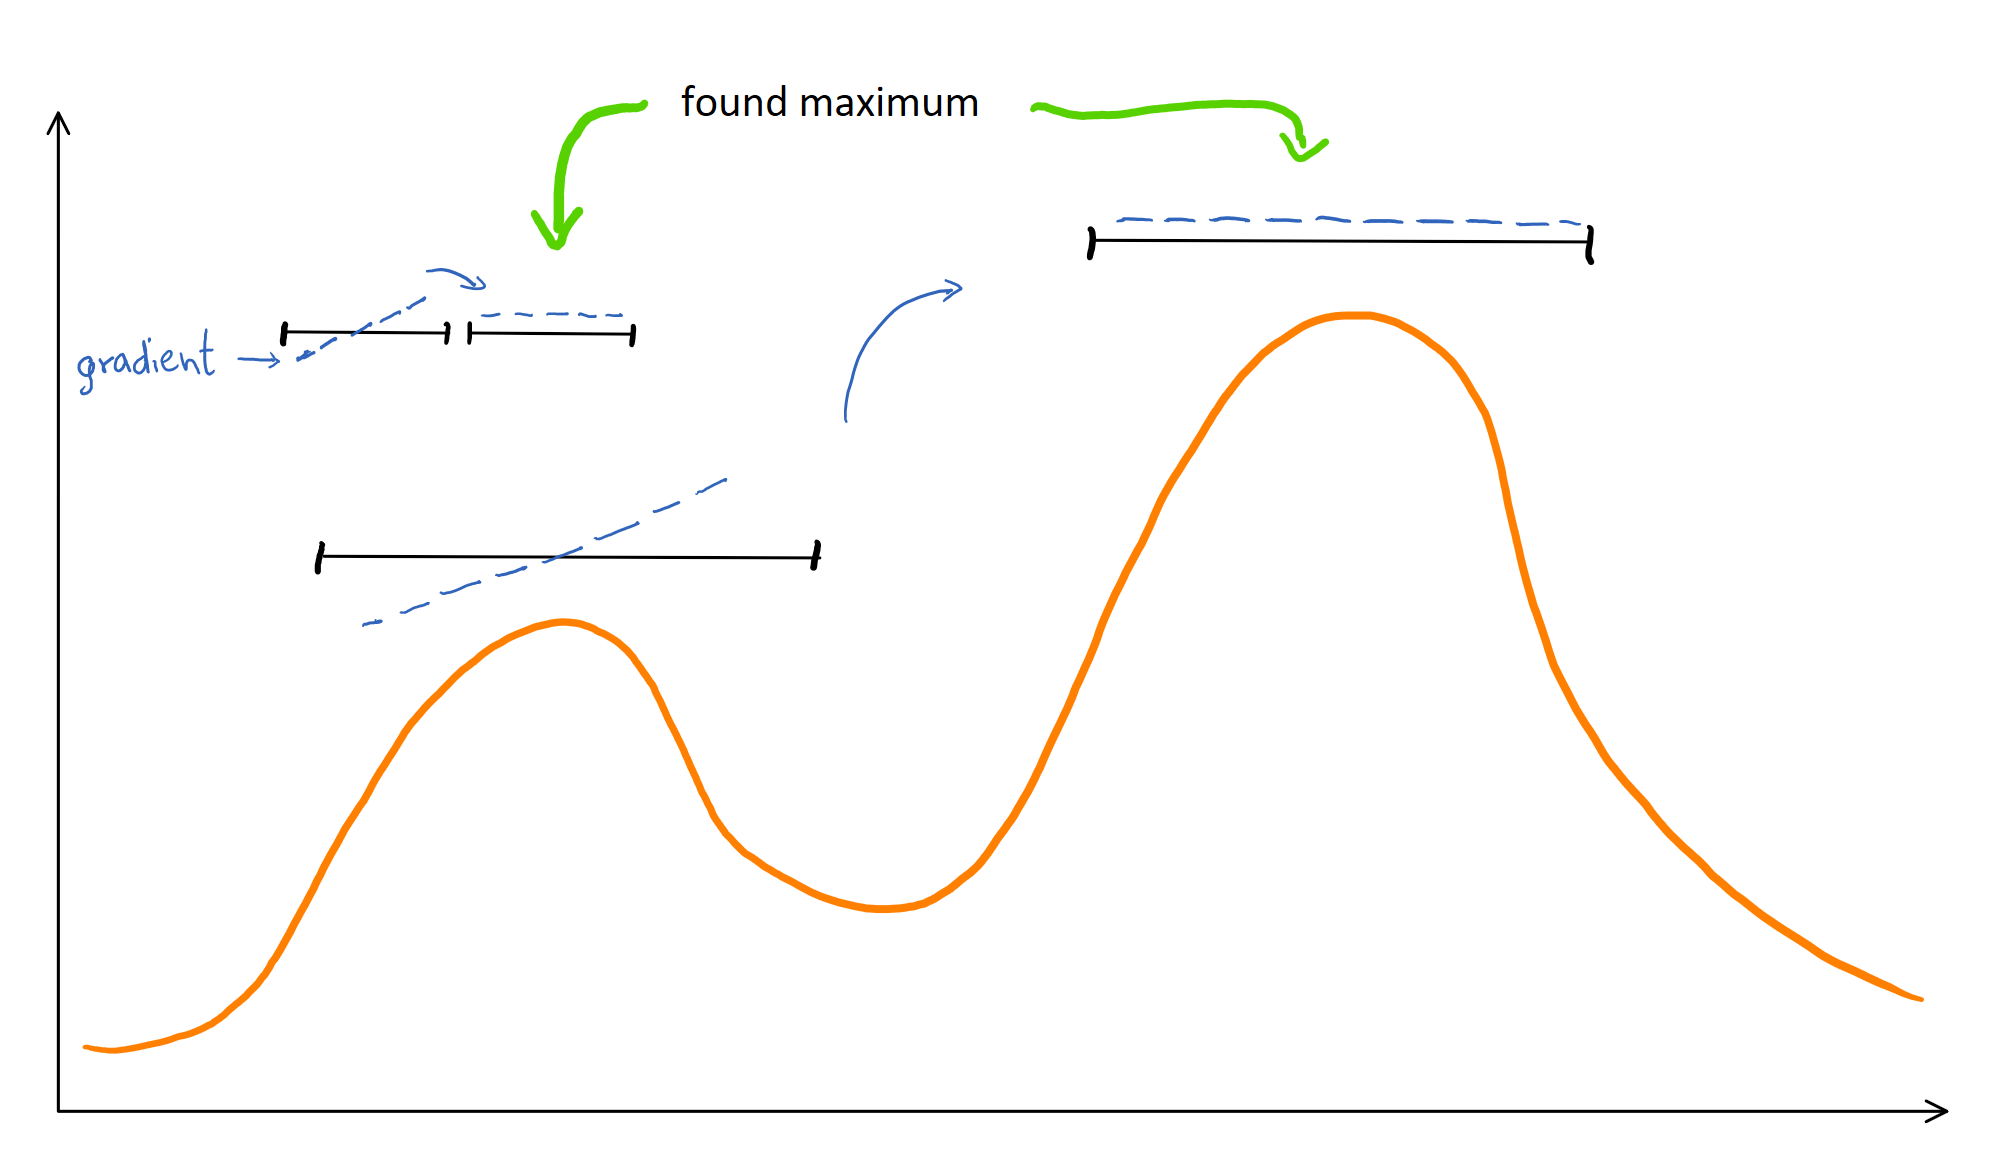
\includegraphics[width=\textwidth]{04-kernel-size}
		\caption{The kernel size h indirectly controls the number of identified maxima}
	\end{minipage}
	\begin{minipage}[b]{0.4\textwidth}
		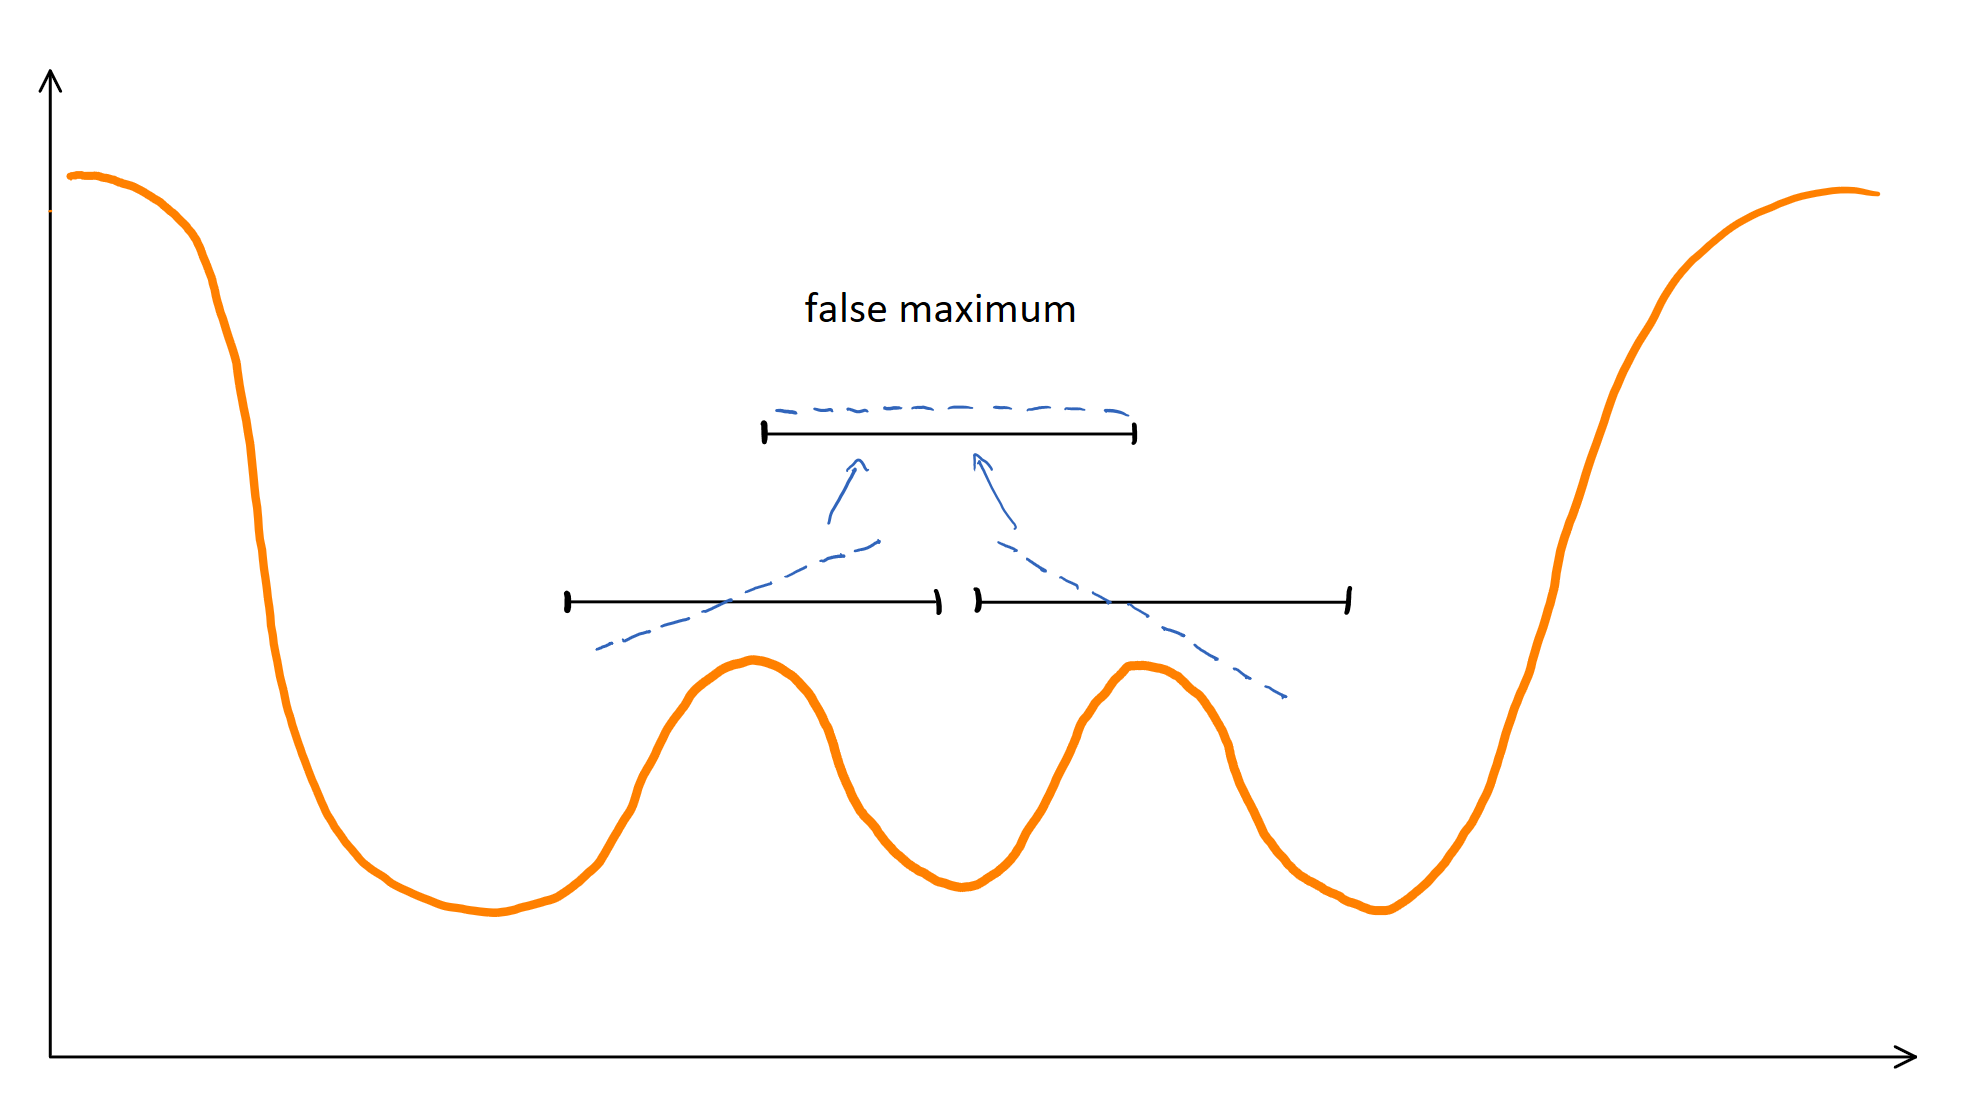
\includegraphics[width=\textwidth]{05-kernel-size-pitfall}
		\caption{One of the issues is, the case when a zero gradient is just between two finer maxima}	
		\label{mean-shift-issue}	
	\end{minipage}
\end{figure}

\subparagraph{Epanechnikov kernel}
If we use the Epanechnikov kernel as $k_h$, then the computation breaks down to the mean of the samples in a circular (hyper-spherical) around $\vec{x}^{(t)}$

\begin{equation*}
  k_E(\vec{x}) = \begin{cases}
    c \cdot (1 - \vec{x}^T \vec{x})&\text{when } \vec{x}^T \vec{x} \le 1\\
    0 &\text{otherwise}
  \end{cases}
\end{equation*}

\begin{figure}[H]
  \centering
  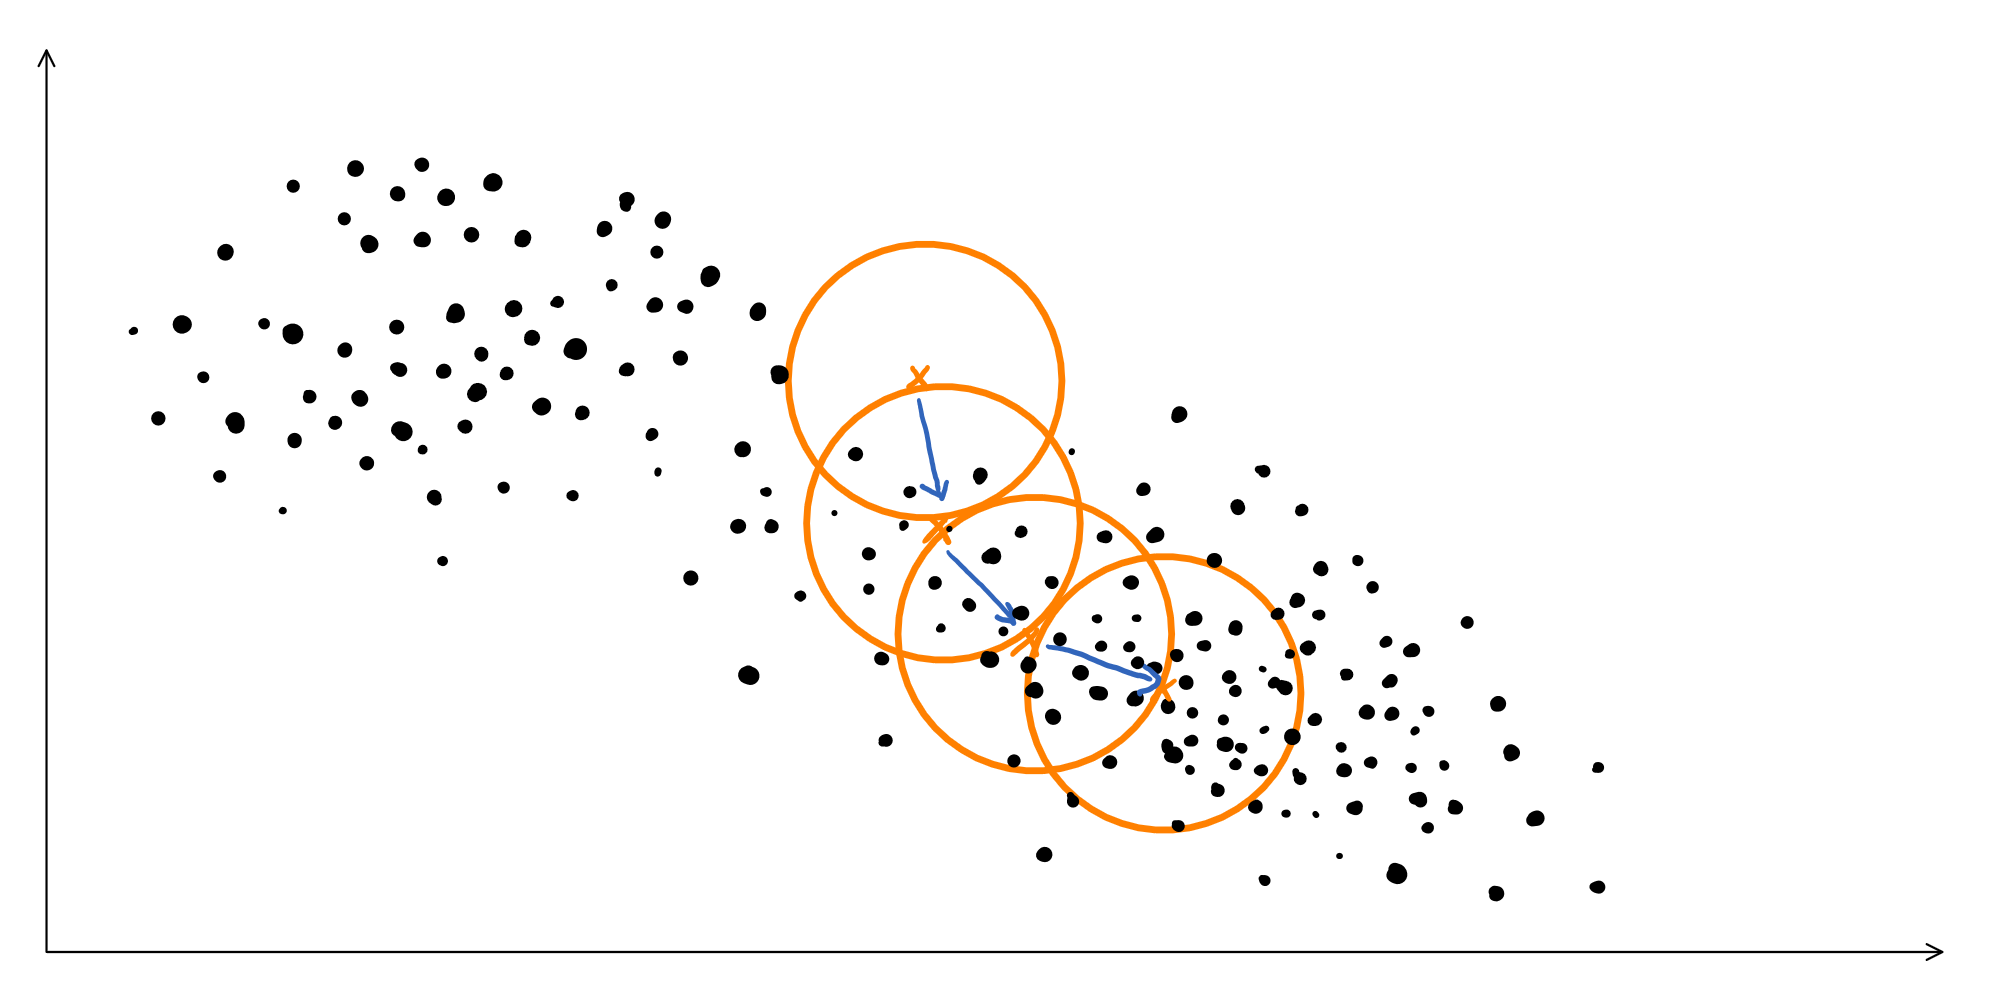
\includegraphics[width=0.4\textwidth]{06-moving-epan-kernel}
  \caption{Mean Shift iterations with an Epanechnikov kernel}
\end{figure}

\subparagraph{Application:}
\begin{itemize}
  \item (Color) quantization: Note, the RGB colorspace is not perceptually uniform (Lab or Luv are used in practice)
  \item (Color) segmentation
    \begin{itemize}
      \item Similar in result to a super pixel segmentation: operates locally in the image
      \item Incorporate the position of each pixel
      \item Properly scale each feature dimension, such that distances are comparable (e.g. $\vec{x} = $(x,y,r,g,b))
    \end{itemize}
\end{itemize}

\subparagraph{Remarks on the found maxima:}
\begin{itemize}
  \item Different trajectories typically coverage only to \textbf{almost} the same peak, thus, we will have to post process the peaks and somehow reduce them.
  \item We don't have a guarantee to sit on top of a maximum when reaching a 0-gradient. This is due to the finite window size and the discrete representation of our density (see figure \ref{mean-shift-issue}).
  \item \label{mean-shift-cost-effectiveness} If the amount of data is large, then it may become extremely costly to iteratively evaluate the ``neighborhood finder''. In that case we have to help ourself, either with a smart data structure (oct-tree or a generalization for many dimensions) or locality sensitive hashing (LSH).
\end{itemize}
